\chapter{Experimental Setup}	\label{chapter:experimental_setup}

MABDI was developed and tested in a completely simulated environment
so that all results could be repeatable and also to facilitate the ability to
debug during the development process. In addition, by performing the analysis in
simulation the global mesh can be visually compared to ground truth.

\section{Simulation Parameters}

The simulation was designed to be highly configurable and is implemented by a
class named MabdiSimulate. The class is initialized with parameters that control
all aspects of the simulation. Parameters of a particular importance are
discussed in more detail here:

\begin{itemize}
    \item Environment - This parameter specifies the environment used to generate
    the simulated depth images. \textit{Table} is an environment consisting of a
    table and two cups placed on the table. The table is 1 meter tall.
    \textit{Bunnies} is an environment consisting of three bunnies who are
    around 1.5 meters tall. These bunnies are created using the Stanford Bunny
    \cite{Turk1994}, a well known data set in computer graphics.
    \item Noise - If true, adds noise to the depth image of the simulated sensor.
    \item Dynamic - If true, adds an object during the simulation. In the case
    of this analysis, a third bunny is added half-way through the simulation.
    \item Iterations - The number of iterations the simulation will have. This
    parameter affects the distance the sensor travels from frame to frame.
\end{itemize}

% parameters chosen the experimental runs
For this paper we will be exploring three experimental runs to demonstrate the
ability of the MABDI implementation to generate valid results. Additionally, the
experimental runs will be able to show the capabilities of the MABDI algorithm
such as handling object addition in the environment.

\begin{table}[h]
  \caption{Description of the experimental runs.}
  \label{tab:run}
  \begin{footnotesize}
  \begin{center}
    \begin{tabular}{|l|c|c|c|c|}
    \hline
           & Environment & Noise   & Dynamic & Iterations \\\hline
    Run 1	 & Table       & False   & False   & 30 \\
    Run 2  & Bunnies     & True    & False   & 50 \\
    Run 3  & Bunnies     & True    & True    & 50 \\
    \hline
    \end{tabular}
  \end{center}
  \end{footnotesize}
\end{table}

All experimental runs define a helical path for the sensor to follow during the
simulation. The path circles the objects in the environment twice. A helical
path was chosen because it returns to a part of the environment that has been
already mapped and is thus ``known'' to the global mesh. Also, because the path
is a helix and not just a circle, the sensor views the environment from a
slightly different position on each pass.

\section{Simulating an RGB-D Sensor}

For the experiments, we simulate a sensor moving in a fixed environment along a
path. The coordinate system fixed to the environment is called the global
coordinate system. The sensor also has a coordinate system attached the origin
of its viewing frustum. The scene is rendered from the sensor's point of view,
and part of the information generated during the rendering process is used as
the output of the simulated sensor. During the rendering process mesh vertices
and elements are transformed from the sensor's coordinate system into view
coordinates using the pinhole camera model. The use of this model has been
validated in the localization work of Fallon \cite{Fallon2012}. The intrinsic
camera parameters of the pinhole hole model were chosen to replicate the Kinect
sensor \cite{sitekinectspecs}. This pinhole camera model transformation takes
everything that is viewable by the sensor and transforms it to a cube placed in
front of the sensor. Each side of this cube has a length of 2 and varies from -1
to 1 along the x, y, and z axis. The x and y values are eventually transformed
into display coordinates, which determine the final pixel locations in the
image. The z values of the cube are normalized from 0 to 1 and define the depth
image.

To simulate a RGB-D sensor, noise is added to the depth image $D$ by
sampling a normal distribution and adding the value to each pixel. as defined in
the equation below.

\begin{equation}
D_{noisy}(i,j) = D(i,j) + \mathcal{N} (\mu\mathsmaller{=}0, \sigma\mathsmaller{=}0.002)
\label{eqn:depth_noise}
\end{equation}

The pinhole camera transformation creates a non-linear relationship between
values in the depth image and their corresponding location in the sensor's
coordinate system. This relationship is visualized in Fig.
\ref{fig:depth_view_to_sensor}. As a consequence, constant noise added to the
depth image grows in magnitude as distance from the sensor increases. Luckily,
this non-linear relation corresponds with RGB-D error models from the
literature. Researchers have created error models to describe the standard
deviation of measurement error found in various RGB-D sensors. For this work, we
seek to match the well-known error model of Khoshelham \cite{Khoshelham2012}
that is based on the original Kinect.

\begin{figure}[h]%[thpb]
\centering
  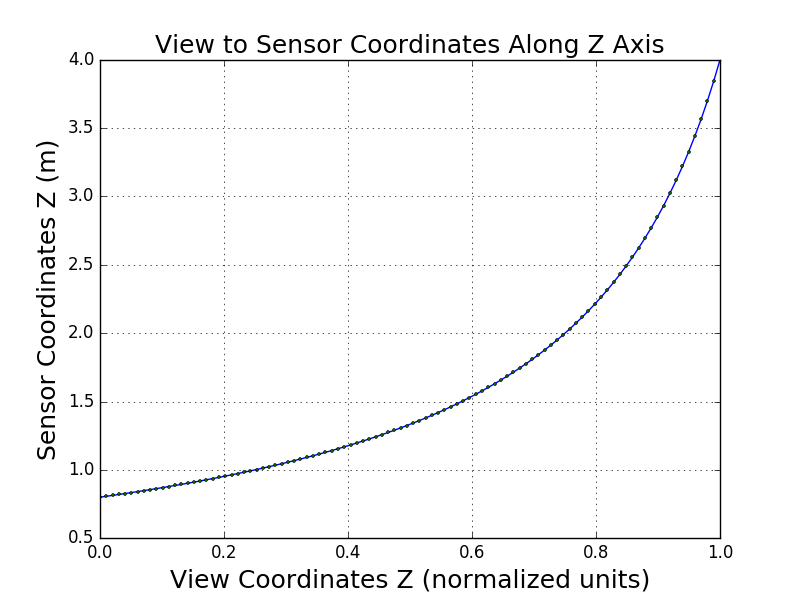
\includegraphics[width=.70\textwidth]{figures/depth_view_to_sensor.png}
  \caption{View coordinates to the sensor's coordinates.}
  \label{fig:depth_view_to_sensor}
\end{figure}

The mean of the normal distribution in Equation \ref{eqn:depth_noise},
$\sigma\mathsmaller{=}0.002$, was experimentally found to provide a conservative
approximation of Khoshelham's error model, which is defined by the equations
below. A visual comparison of the standard deviation of error used in MABDI's
simulation of a RGB-D sensor and Khoshelham's error model can be seen in Fig.
\ref{fig:depth_noise_error}. From the graph, we can see that the error used in
the simulation is larger than that of the error model and thus have confidence
of MABDI's ability to work in the real world.

\begin{gather}
  \sigma_z = \sigma_d \times \frac{m}{fb} \times Z^2 \\
  \sigma_d = 0.5 \\
  \frac{m}{fb} = 2.85\mathrm{e}{-5}
\end{gather}

\begin{figure}[h]%[thpb]
\centering
  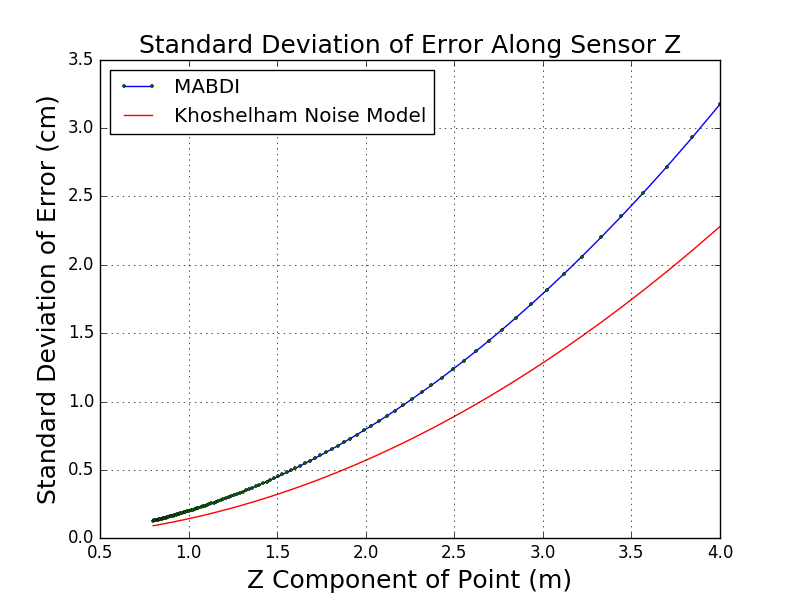
\includegraphics[width=.70\textwidth]{figures/depth_noise_error.png}
  \caption{Comparison of standard deviation of the error used in the MABDI simulation and the error model from Khoshelham.}
  \label{fig:depth_noise_error}
\end{figure}
